\documentclass[11pt]{article}
\usepackage[margin=0.8in]{geometry}
\usepackage{graphicx}
\usepackage{booktabs}
\usepackage{array}
\usepackage{float}
\title{NV23 image231924 c01 closeout: aligned NV, Ramsey $T_2^*$, and $^{13}$C check}
\author{OpenClaw nv-researcher}
\date{2026-05-12}
\begin{document}
\maketitle

\section*{Executive summary}
The project objective was to find a magnetic-field-aligned NV in the image231924
spatial range, then obtain a well-supported Ramsey $T_2^*$ and $^{13}$C conclusion.
The first candidate, \texttt{image231924\_c01}, was trackable and passed the requested
strong-pi pulsed ODMR alignment screen. Weak-pi pulsed ODMR refined the microwave
center, and a corrected-center Ramsey repeat completed normally. The terminal
conclusion is:

\begin{itemize}
\item Magnetic-field-aligned NV found: \texttt{image231924\_c01}.
\item Ramsey signal: present, with a repeatable oscillatory component near 1.76 MHz.
\item $T_2^*$: supported scale about $4.0~\mu\mathrm{s}$ from a Gaussian-envelope Ramsey fit; model-dependent range from exponential/stretched/Gaussian fits is approximately $3.2$--$4.0~\mu\mathrm{s}$. This is a scale estimate, not sub-100-ns precision.
\item $^{13}$C: no resolved nearby $^{13}$C coupling is supported by the corrected-center Ramsey FFT. The data do not show a clean carrier plus symmetric \(\mathrm{det}\pm f_{^{13}\mathrm{C}}\) sideband pair; the lower target bin is embedded in a broad carrier/detuning-like band and the upper target bin is weak.
\end{itemize}

\section*{Evidence chain}
\begin{tabular}{@{}>{\raggedright\arraybackslash}p{0.22\linewidth}>{\raggedright\arraybackslash}p{0.45\linewidth}>{\raggedright\arraybackslash}p{0.25\linewidth}@{}}
\toprule
Step & Result & Main evidence \\
\midrule
Image export and seed & Explicit image-axis contract; c01 seed selected & candidate list JSON \\
TrackCenter & c01 passed, 36.008 kcps first pass & bridge result 23:36 \\
Strong-pi pODMR retry & Visible resonance near 3.879 GHz, 23--25\% normalized dip & analysis 00:38 \\
Weak-pi pODMR & Usable center 3.8758666667 GHz, grid-limited & analysis 01:16 \\
First Ramsey scout & Oscillation present; T2*/13C ambiguous & analysis 02:49 \\
Narrow weak-pi refresh & Updated center 3.8761166667 GHz & analysis 03:17 \\
Corrected-center Ramsey & Terminal T2*/13C closeout & analysis 05:18 \\
\bottomrule
\end{tabular}

\section*{Terminal Ramsey acquisition}
The terminal corrected-center Ramsey job was the 03:21 EDT execute for c01. It ran
\texttt{ramsey.xml} with \(\tau=0\ldots8~\mu\mathrm{s}\), 51 points, 6 averages, and
100000 repetitions per average. The bridge completed normally at 04:51 EDT.
Auto-align counts were 23.416 kcps and post-run final counts were 26.645 kcps.
The saved experiment is the 2026-05-12 03:24:49 Ramsey savedexperiment.

The review used raw readouts plus two normalized views: point-wise \(r_2/r_1\) and
signal divided by a linear fit to readout 1. The sequence metadata identifies
readout 1 as the pre-Ramsey \(m_S=0\) reference and readout 2 as the post-Ramsey
signal for \texttt{full\_experiment=0}.

\begin{figure}[H]
\centering
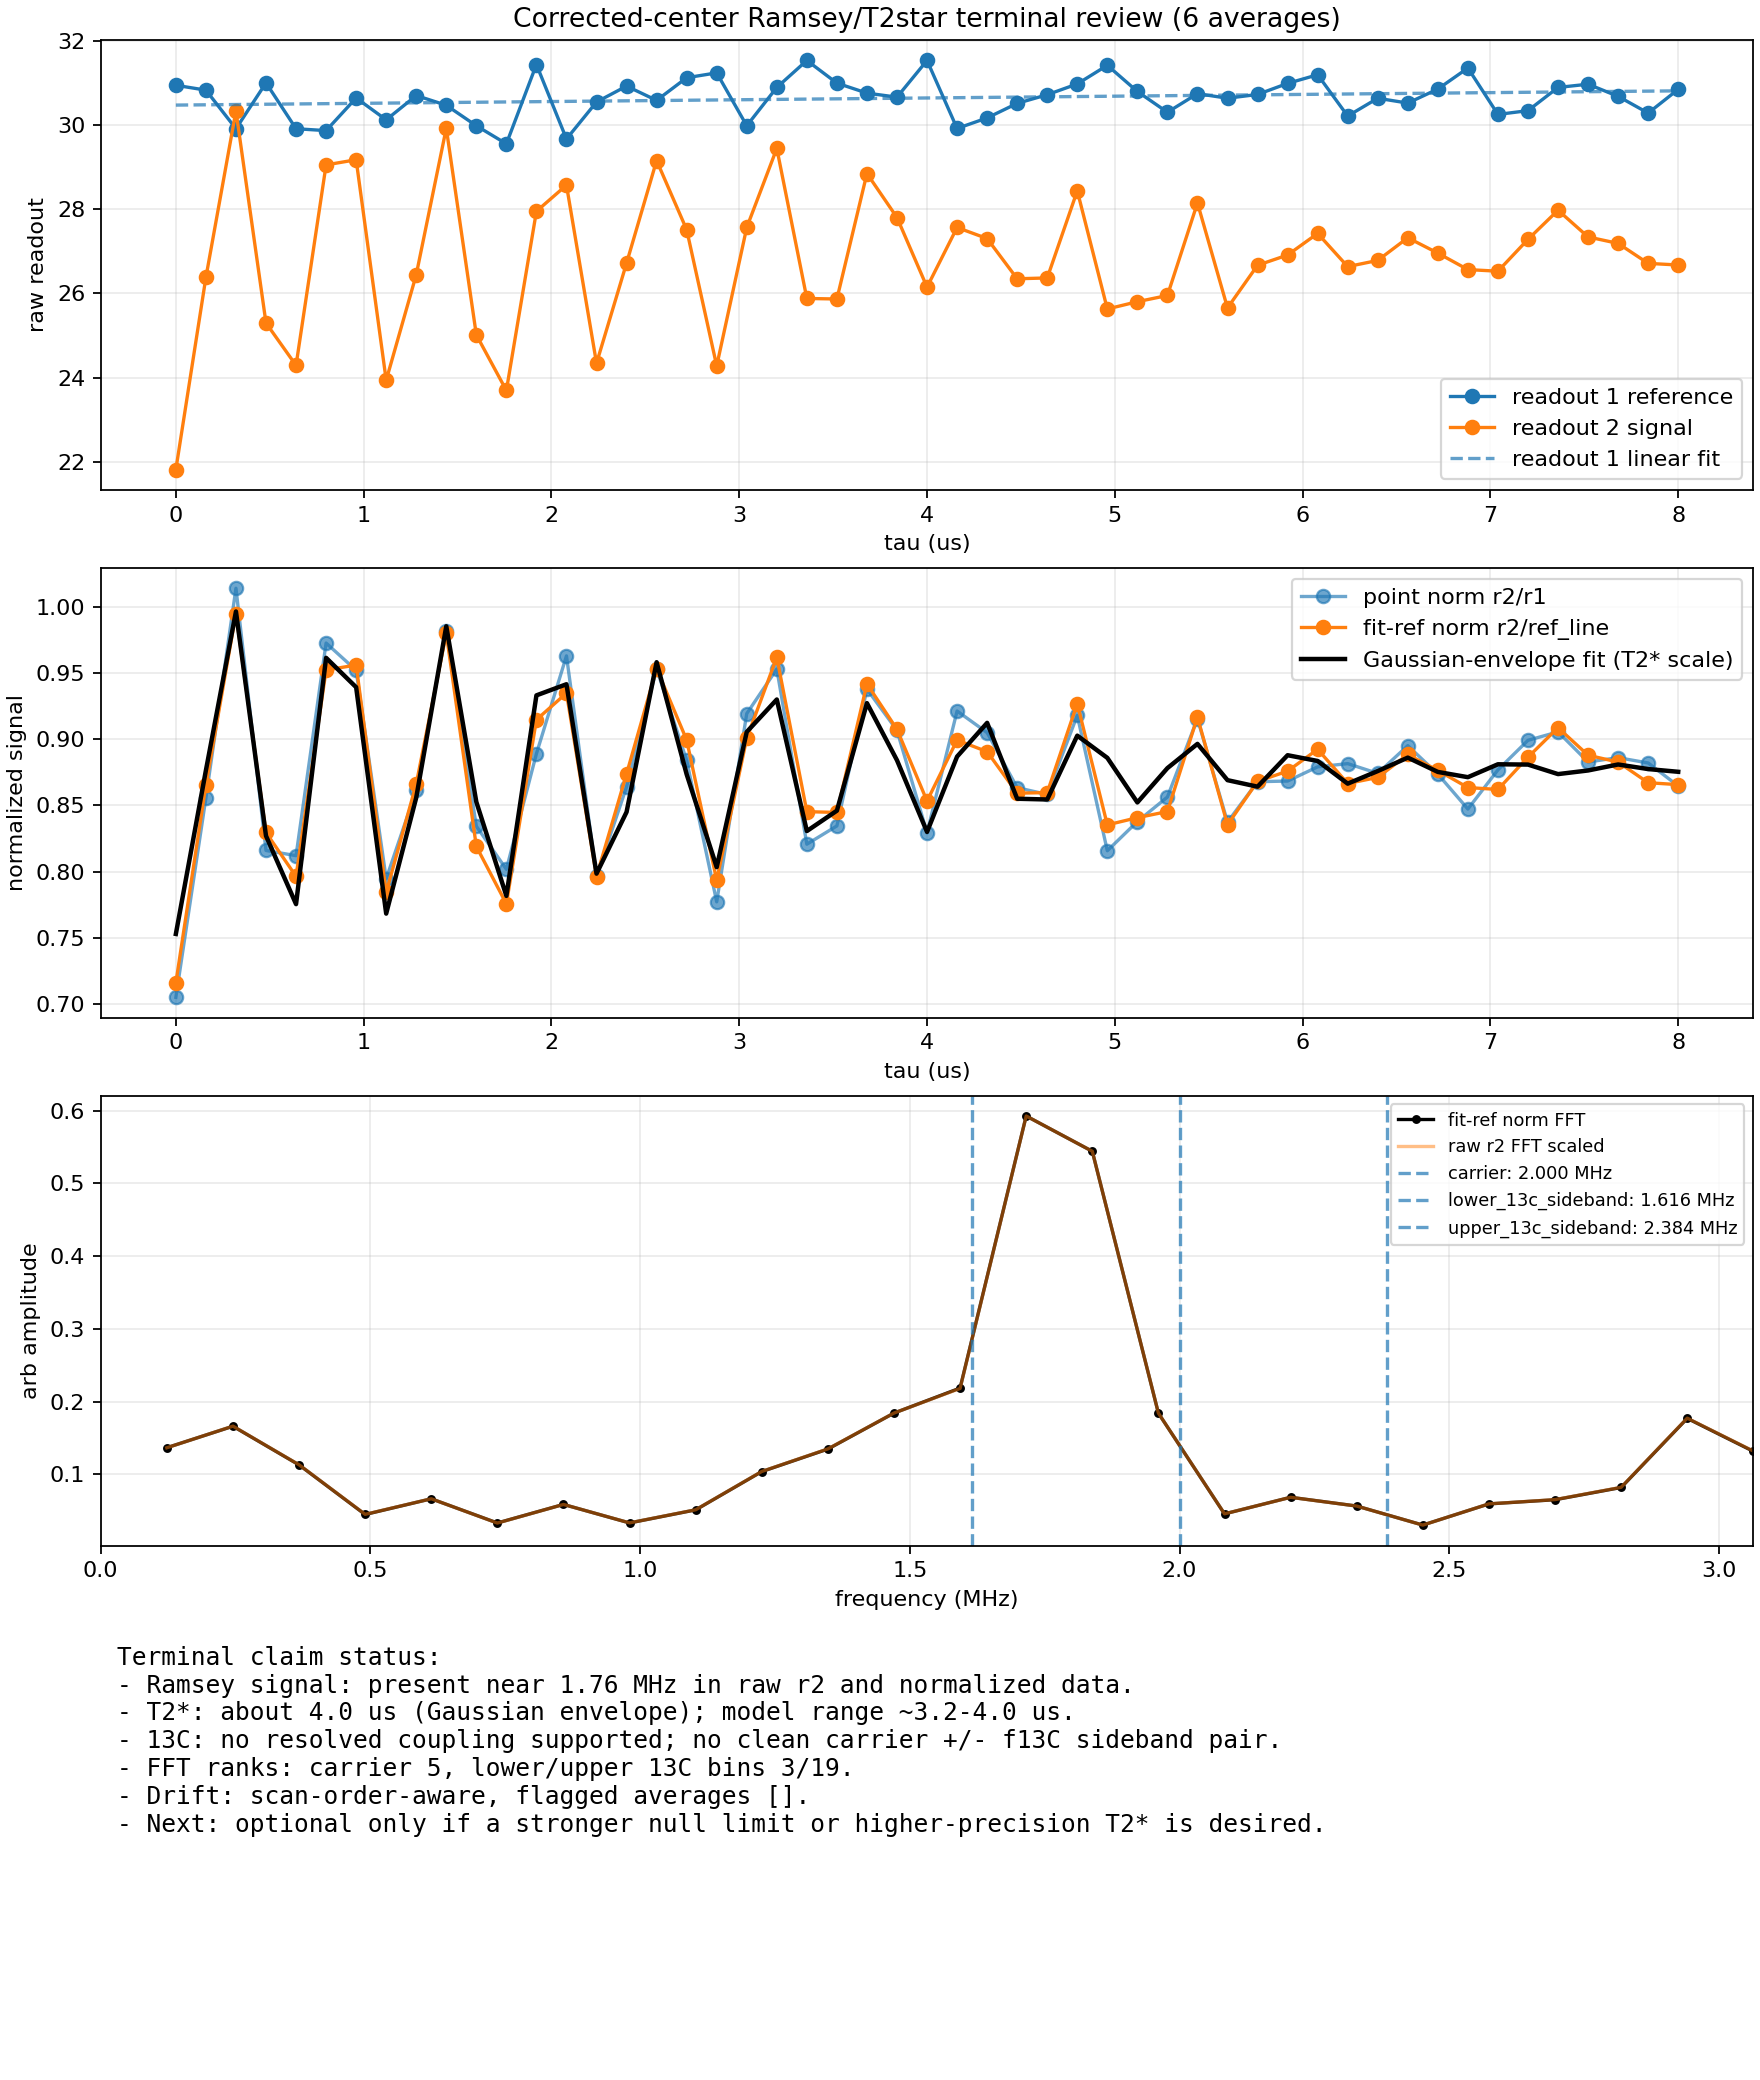
\includegraphics[width=0.98\linewidth]{figures/terminal_review.png}
\caption{Terminal corrected-center Ramsey review. The top panel shows raw readouts, the middle panel shows normalized signal and the Gaussian-envelope fit, and the bottom panel shows the FFT with planned carrier and $^{13}$C sideband markers.}
\end{figure}

\section*{$T_2^*$ assessment}
The Ramsey oscillation is visible in raw readout 2 and in fitted-reference-normalized
signal. The two largest FFT bins are 1.716 MHz and 1.838 MHz, with an
amplitude-weighted center near 1.774 MHz. Stored-average support is moderate and
consistently positive: 15 pairwise detrended normalized-trace correlations have
median 0.571 and range 0.375--0.659.

The preferred empirical fit is a Gaussian-envelope Ramsey decay on the
fitted-reference-normalized signal. It gives
\[
T_2^* \approx 4.03~\mu\mathrm{s}, \qquad f \approx 1.759~\mathrm{MHz}.
\]
An exponential-envelope fit gives \(T \approx 3.16~\mu\mathrm{s}\), and a stretched
fit gives \(T \approx 3.89~\mu\mathrm{s}\) with stretch exponent about 1.70. The
project should therefore report a supported $T_2^*$ scale of about
\(4~\mu\mathrm{s}\), with model-dependence at the few-tenths-to-one-microsecond level.

\begin{figure}[H]
\centering
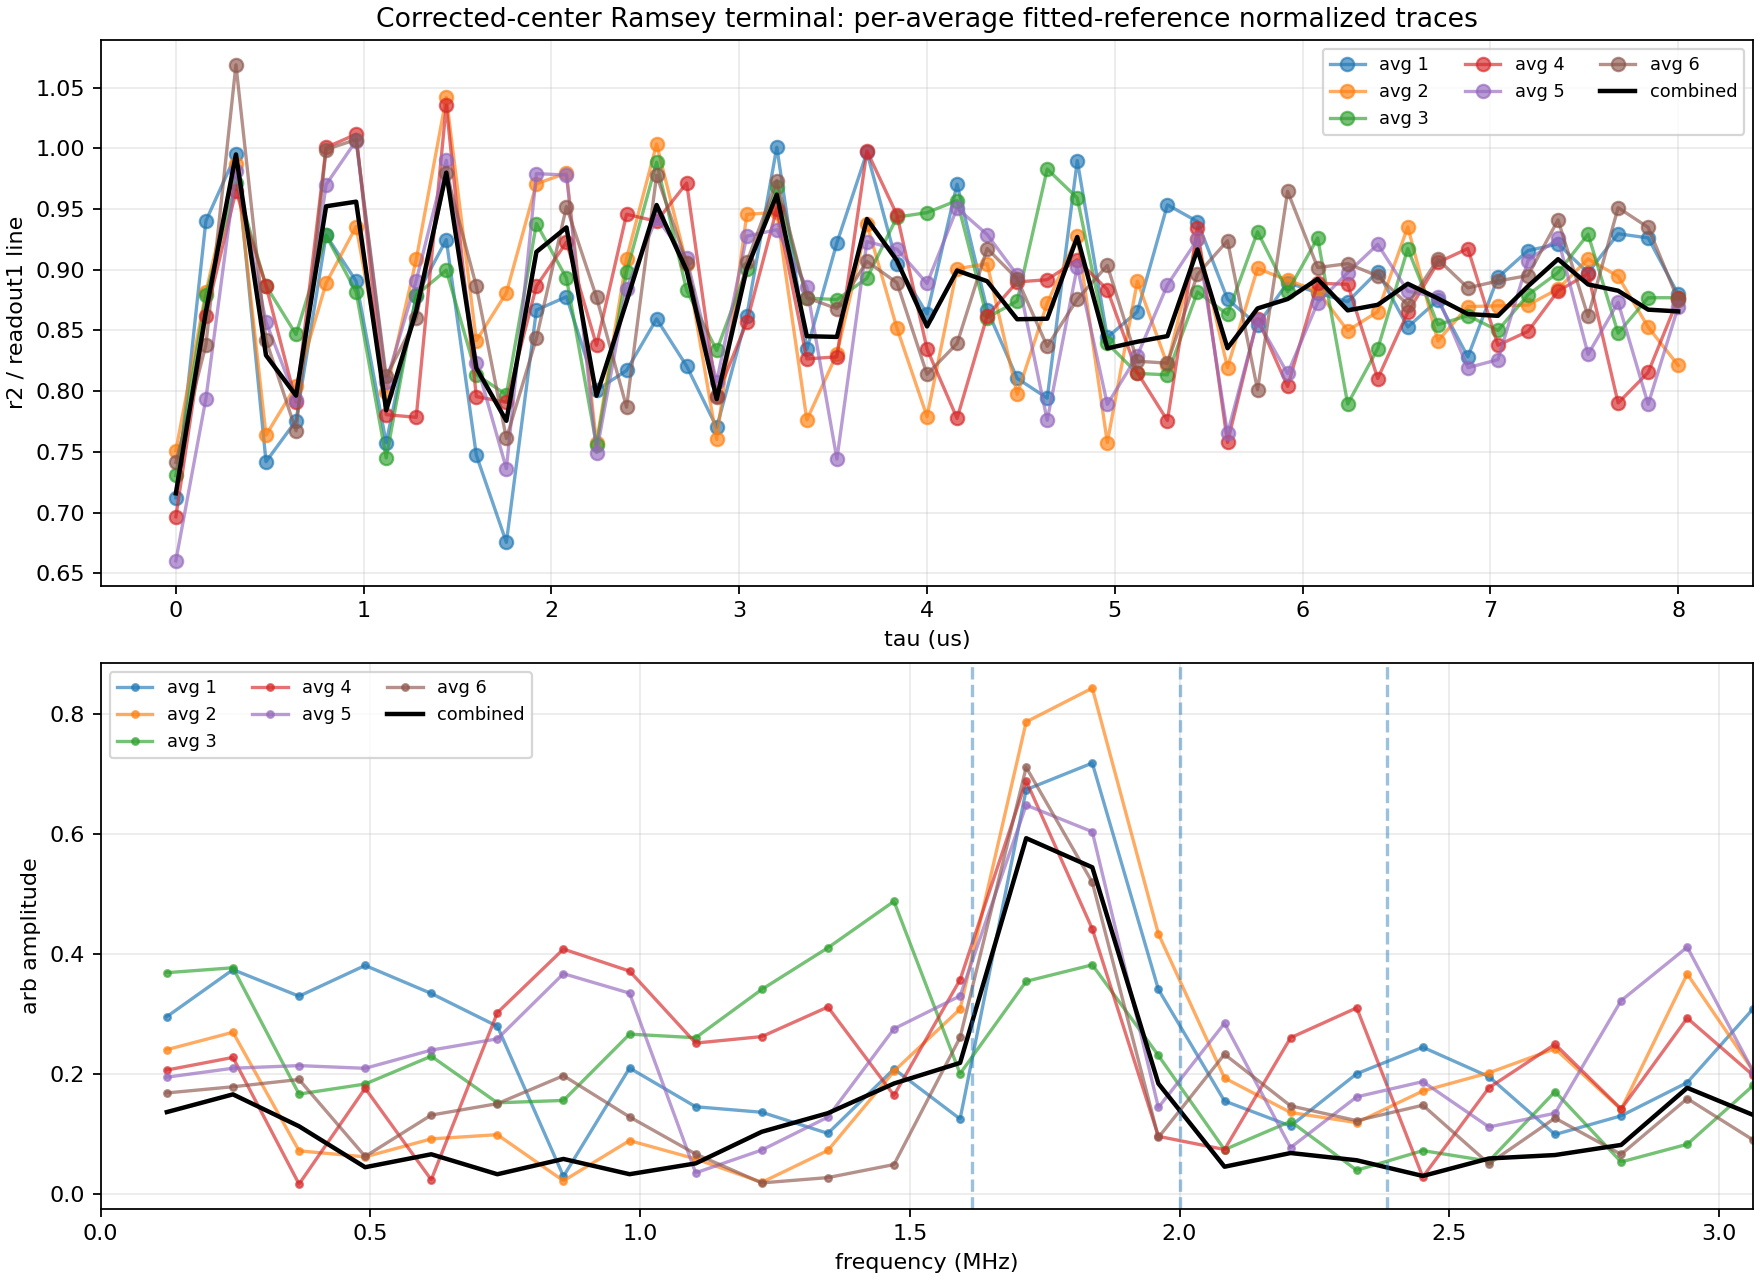
\includegraphics[width=0.98\linewidth]{figures/terminal_per_average.png}
\caption{Per-average normalized Ramsey traces and FFTs. The dominant band is visible across stored averages, supporting a real Ramsey signal rather than a one-average artifact.}
\end{figure}

\section*{$^{13}$C assessment}
Using the weak-pi center and the project planning model, the expected $^{13}$C
Larmor scale was about 384 kHz. For the 2 MHz Ramsey detuning, the expected FFT
markers were therefore near 1.616 MHz, 2.000 MHz, and 2.384 MHz. In the terminal
fitted-reference-normalized FFT, the carrier target bin ranks 5, the lower
$^{13}$C target bin ranks 3, and the upper target bin ranks 19.

This is not a claim-grade $^{13}$C signature. The lower target bin is present, but
it is part of a broad carrier/detuning-like band centered around 1.76--1.84 MHz.
The upper target bin is weak, and the data do not show a clean symmetric sideband
pair around a resolved carrier. The supported conclusion is therefore: no resolved
nearby $^{13}$C coupling is observed in the corrected-center Ramsey data. This is a
negative claim at the current measurement sensitivity and analysis scope, not a
proof that no nuclear spin exists anywhere near the NV.

\section*{Drift and data-quality checks}
The scan-order-aware drift diagnostic used \texttt{Scan.ScanOrderEachAvg} in snake
mode for all 6 averages and flagged no averages. Raw readout 1 changed slowly and
was handled by fitted-reference normalization; raw readout 2 and normalized views
agree on the main oscillatory band. The signal amplitude is large compared with the
FFT non-DC median noise floor, but the exact $T_2^*$ value remains model-dependent.

\begin{figure}[H]
\centering
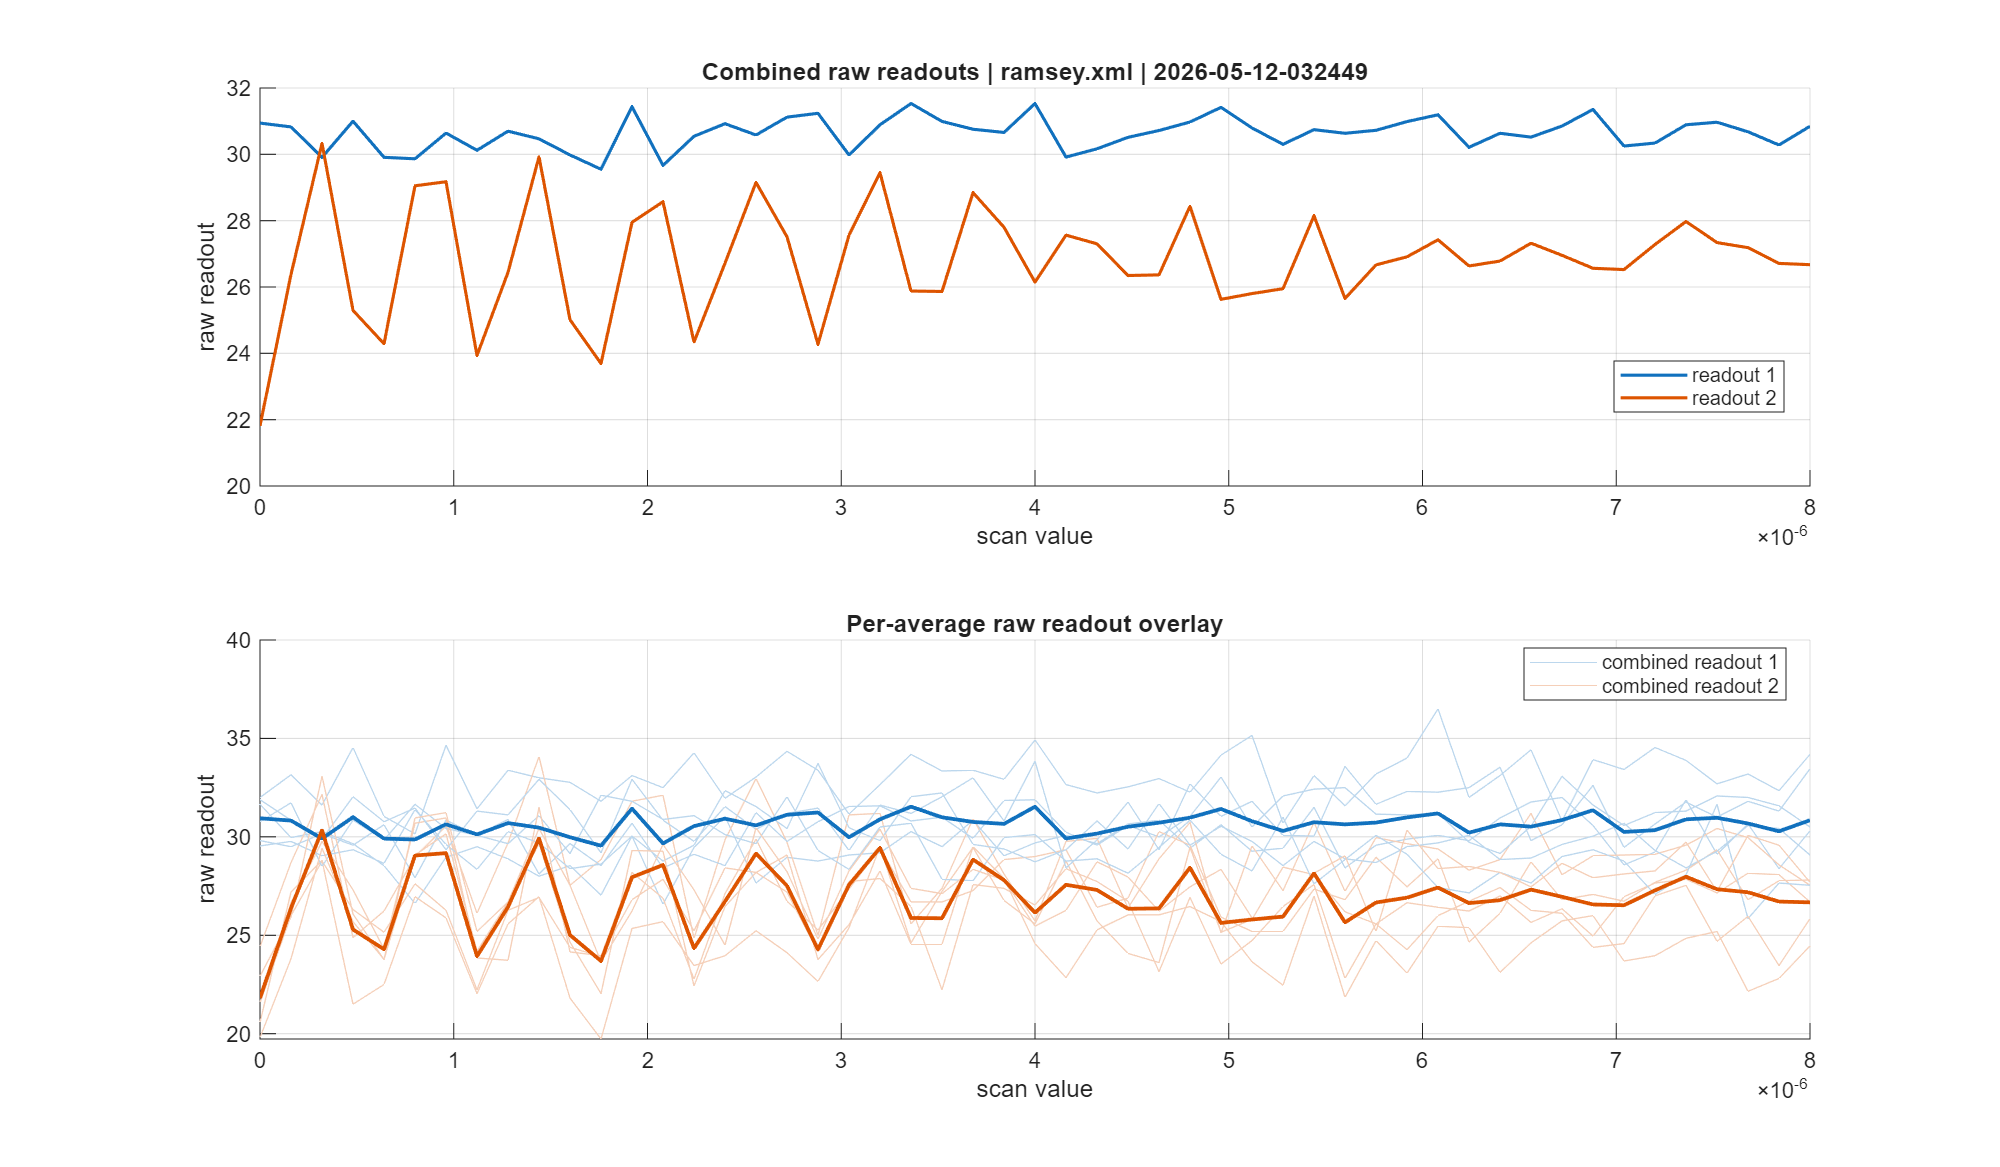
\includegraphics[width=0.98\linewidth]{figures/terminal_raw_readouts.png}
\caption{Raw readout export diagnostic for the terminal Ramsey savedexperiment.}
\end{figure}

\section*{Literature and prior-result context}
The default NV reference in the local literature library is Doherty et al.,
``The nitrogen-vacancy colour centre in diamond,'' Physics Reports 528, 1--45
(2013), DOI 10.1016/j.physrep.2013.02.001. Crossref metadata for this DOI was
checked on 2026-05-12. The project used the standard aligned-band planning
approximation to estimate the field and $^{13}$C Larmor frequency; the exact
calculation is recorded in
\texttt{work/notes/image231924\_c01\_ramsey\_fft\_expectation\_20260512\_0130.md}.

\section*{Closeout decision}
The human objective is satisfied for \texttt{image231924\_c01}: a magnetic-field-aligned
NV was found, $T_2^*$ has a supported scale, and the $^{13}$C check has a supported
negative conclusion at the current measurement sensitivity. Further bridge work is
optional only if operator wants a higher-precision $T_2^*$ estimate or a stronger
null limit on weak $^{13}$C coupling.

\end{document}

